\chapter{Implementierung der automatisierten Testinfrastruktur}

Das Endziel dieser Arbeit ist die Einrichtung einer automatisierten
Testinfrastruktur, um die Webanwendung jExam und ihre zukünftige
Version, die sich noch in der Entwicklung befindet, zu testen.
Dabei sollen nicht nur die wichtigsten
Funktionen getestet werden, sondern auch die Sicherheit und die
Performance. Dieses Kapitel konzentriert sich auf die Einrichtung
dieser Testinfrastruktur sowie auf das Design und die Entwicklung
der Tests. Außerdem werden die verschiedenen verwendeten Technologien
vorgestellt und ihre Verwendung begründet.


\section{Vorstellung der Testansatzes}

Die jExam-Webanwendung muss auf drei verschiedenen Ebenen getestet
werden: Funktionalitäten, Performance und Sicherheit. Es ist jedoch
nicht möglich, diese drei Ebenen in einer einzigen Testsuite zu
kombinieren. Dies erfordert die Einrichtung einer Infrastruktur,
die die Erstellung und Ausführung der Tests verwaltet. Die Anwendung,
die verwendet wird, um die verschiedenen Dienste zu trennen, ist Docker \cite{docker}
(wird in den folgenden Kapiteln behandelt). Docker  wird nicht nur für
die Trennung der Testebenen verwendet. Sie ermöglicht es auch, beide
Versionen von jExam zu deployen, sodass sie effizient und lokal
getestet werden können. Über diese Infrastruktur wird es möglich
sein, Tests auszuführen und am Ende ihrer Ausführung Berichte und
Metriken zu erhalten. Über diese Infrastruktur wird es möglich sein,
Tests auszuführen und am Ende ihrer Ausführung Berichte und Metriken
zu erhalten. Diese ermöglichen , die Leistung der beiden Plattformen
zu beobachten und zu vergleichen. In den nächsten Kapiteln werden
alle diese Konzepte im Detail behandelt.


\section{Entwicklung von Sicherheitstests}

\subsection{\acs{owasp}}

\acs{owasp} ist das Akronym für \textbf{O}pen \textbf{W}eb
\textbf{A}pplication \textbf{S}ecurity \textbf{P}roject und
beschreibt eine offene Organisation, deren Hauptziel ist, die
Sicherheit von Anwendungen, Diensten und Software zu verbessern.
Sie wurde am 1. Dezember 2001 gegründet und am 21. April 2004 als
gemeinnützige Organisation offiziell anerkannt.  Sie ermöglicht
Organisationen, Unternehmen oder Einzelpersonen, sichere Anwendungen zu
entwickeln und zu warten. Die \acs{owasp} hat eine Reihe von
Sicherheitstools und -richtlinien entwickelt. Dazu gehören die \acs{owasp}
Top 10 und der Zed Attack Proxy (\acs{zap}). Ein wichtiger
Grundsatz der OWASP ist, dass jeder, der sich für die Sicherheit
von Webanwendungen interessiert, weltweit kostenlos über das
nötige Wissen und die Werkzeuge verfügen kann (vgl. \cite{owasp}).
In diesem Zusammenhang hat sie die OWASP TOP 10 erstellt, die eine
Liste der zehn häufigsten Sicherheitslücken im Internet
darstellt. Ihr Hauptzweck ist die Schulung all jener, die mit der
Entwicklung sicherer Anwendungen zu tun haben.  Sie sollen über die
üblichsten Sicherheitslücken informiert werden und dadurch diese
vermeiden.  Im Folgenden werden die zehn Angriffe der OWASP TOP
10 auf der Basis der OWASP TOP 10 2017 
Release Candidate 2 (vgl. \cite{Stock2017}) beschrieben.

\begin{table}[h]
    \begin{tabulary}{\textwidth}{@{}L@{}}
        \toprule
        \textbf{OWASP TOP10 2017} \tabularnewline\midrule
        1"~ Injektion (Injection)
        \tabularnewline
        2"~ Fehler in der Authentifizierung (Broken Authentication)
        \tabularnewline
        3"~ Verlust der Vertraulichkeit von Daten (Sensitive Data Exposure)
        \tabularnewline
        4"~ XML External Entities (XML)
        \tabularnewline
        5"~ Fehler in der Zugriffskontrolle (Broken Access Control)
        \tabularnewline
        6"~ Sicherheitsrelevante Fehlkonfiguration (Security Misconfiguration)
        \tabularnewline
        7"~ Cross-Site-Scripting (XSS)
        \tabularnewline
        8"~ Unsichere Deserialisierung (Insecure Deserialization)
        \tabularnewline
        9"~ Nutzung von Komponenten mit bekannten Schwachstellen (Using Components with Known Vulnerabilities)
        \tabularnewline
        10"~ Unzureichendes Logging und Monitoring (Insufficient Logging and Monitoring)
        \tabularnewline\bottomrule
    \end{tabulary}
    \caption{OWASP TOP 10 2017}\label{tab:OWASP_TOP_10}
\end{table}

\subsubsection{Injektion}

Eine Injektion ist eine Schwachstelle, die einem Angreifer ermöglicht,
bösartigen Code durch eine Anwendung auf ein anderes System zu
schleusen. Dabei können sowohl Backend-Systeme als auch andere
Clients, die mit der angreifbaren Anwendung verbunden sind, gefährdet
werden. Zu den Auswirkungen dieser Angriffe gehören:

\begin{enumerate}
    \item Einem Angreifer erlauben, Betriebssystemaufrufe auf einem
    Zielrechner auszuführen.
    \item Einem Angreifer ermöglichen, Backend-Datenspeicher
    zu kompromittieren.
    \item Einem Angreifer ermöglichen, die Sitzungen anderer
    Benutzer zu kompromittieren oder umzuleiten.
    \item Einem Angreifer erlauben, Aktionen im Namen anderer
    Benutzer oder Dienste zu erzwingen.
\end{enumerate}

Viele Webanwendungen hängen von Betriebssystemfunktionen, externen
Programmen und der Verarbeitung von Datenabfragen ab, die von
Benutzern eingereicht werden. Wenn eine Webanwendung Informationen
aus einer HTTP-Anfrage als Teil einer externen Anfrage weitergibt,
sollten Sie eine Möglichkeit zur Überprüfung und Validierung der
Nachricht einrichten. Andernfalls kann ein Angreifer spezielle
(Meta-) Zeichen, bösartige Befehle/Codes oder Befehlsmodifikatoren in
die Nachricht einfügen. Diese Angriffe sind zwar nicht schwer
auszuführen, aber es gibt immer mehr Tools, die nach diesen
Fehlern suchen. Ein Angreifer kann diese Techniken nutzen, um den
Inhalt Ihrer Datenbank zu erhalten, zu beschädigen oder zu zerstören,
Backend-Systeme zu kompromittieren oder andere Benutzer anzugreifen.
Erfolgreiche Injektionsangriffe können ein System vollständig
gefährden oder zerstören. Es ist wichtig, auf diese Arten von
Angriffen zu testen und sich dagegen zu schützen.

Als Beispiel kann man die SQL-Injektion nennen. Diese ist eine
besonders weit verbreitete und gefährliche Form der Injektion.
Um einen SQL-Injektion-Fehler auszunutzen, muss ein Angreifer
einen Parameter finden, den die Webanwendung an eine
Datenbankinteraktion weitergibt. Ein Angreifer kann dann
bösartige SQL-Befehle in den Inhalt des Parameters einbetten.
Das bringt die Webanwendung dazu, eine bösartige Abfrage an die
Datenbank weiterzuleiten. SQL-Abfragen könnten durch Hinzufügen
zusätzlicher ``Einschränkungen'' zu einer Anweisung (z. B. OR 1=1)
geändert werden, um Zugriff auf nicht autorisierte Daten zu
erhalten oder diese zu ändern.



\subsubsection{Fehler in der Authentifizierung}

Wenn die Authentifizierungsfunktionen  einer Anwendung nicht korrekt
implementiert sind, können Angreifer Passwörter oder Sitzungs-IDs
kompromittieren oder andere Implementierungsfehler ausnutzen, indem
sie die Anmeldedaten anderer Benutzer verwenden. Diese Schwachstelle
wird als ``Fehler in der Authentifizierung'' (Broken authentication
in Englisch) bezeichnet. Es wird in der Regel durch schlecht
implementierte Authentifizierungs- und Sitzungsverwaltungsfunktionen
verursacht. In diesem Fall  zielen Angriffe darauf ab, die Kontrolle
über ein oder mehrere Benutzerkonten zu erlangen, indem der Angreifer
die gleichen Privilegien erhält wie der angegriffene Benutzer.
Es wird vom ``Fehler in der Authentifizierung'' besprochen ,
wenn Angreifer in der Lage sind, Passwörter, Schlüssel oder
Sitzungs-Tokens, Benutzerkontoinformationen und andere
Details zu kompromittieren, um Benutzeridentitäten zu übernehmen.
Zu den üblichen Risikofaktoren gehören:


\begin{enumerate}
    \item Vorhersehbare Anmeldekennungen
    \item Benutzerauthentifizierungskennungen, die nicht geschützt sind, wenn sie gespeichert werden.
    \item Sitzungs-IDs, die in der URL offengelegt werden (z. B. durch URL-Rewriting).
    \item Sitzungs-IDs, die anfällig für Session-Fixing-Angriffe sind.
    \item Sitzungswert, der nach dem Abmelden nicht unterbrochen oder ungültig gemacht wird.
    \item Sitzungskennungen, die nach einer erfolgreichen Anmeldung nicht erneuert werden.
    \item Passwörter, Sitzungskennungen und andere Identifikationsinformationen, die über unverschlüsselte Verbindungen gesendet werden.
\end{enumerate}
\subsubsection{Verlust der Vertraulichkeit von Daten}

Der Verlust der Vertraulichkeit von  Daten tritt auf, wenn eine
Organisation unwissentlich sensible Daten offenlegt oder wenn ein
Sicherheitsvorfall dazu führt, dass sensible Daten versehentlich
oder rechtswidrig zerstört, verloren, verändert, unbefugt
offengelegt oder unbefugt darauf zugegriffen wird. Eine solche
Datenexposition kann das Ergebnis eines unzureichenden Schutzes einer
Datenbank, einer Fehlkonfiguration bei der Erstellung neuer Instanzen
von Datenspeichern oder einer unsachgemäßen Nutzung von Datensystemen sein.

Klassische Beispiele dafür sind in Klartext gespeicherte Daten, wie
Passwörter oder Kreditkartendaten, fehlendes HTTPS auf
authentifizierten Webseiten, und Hash-Passwörter, die ohne zugefügtes
“Salz” erstellt wurden. Salz bezeichnet eine zufällige Zeichenfolge,
die den Klardaten vor der Verschlüsselung hinzugefügt werden. Dadurch
kann anhand identischer Hashwerte nicht darauf geschlossen werden,
dass es sich um dieselben Daten handelt.
\subsubsection{XML External Entities (XML)}

\acs{xml} External Entity Injection (auch bekannt als \acs{xee}) ist eine
Sicherheitslücke, die einem Angreifer ermöglicht, in die Verarbeitung
von \acs{xml}-Daten durch eine Anwendung einzugreifen. Dieser Angriff
erfolgt, wenn die \acs{xml}-Eingabe, die einen Verweis auf eine externe
Entität enthält, von einem schwach konfigurierten \acs{xml}-Parser
verarbeitet wird. Dieser Angriff kann zur Offenlegung vertraulicher
Daten, Denial of Service, serverseitiger Anfragefälschung,
Portanalyse aus der Sicht des Computers, auf dem sich der Parser
befindet, und anderen Auswirkungen auf das System führen. Um \acs{xxe}
Injections zu verhindern, sollen folgende Punkte beachtet werden:


\begin{enumerate}
    \item Einfachere Datenformate wie JSON zur Datenübertragung verwenden.
    \item Das Verbot in allen \acs{xml}-Parsern, \acs{xml}-Entitäten
     und \acs{dtd}s verändern. \acs{dtd} steht für Document Type Definition und
     bezeichnet einen XML Dokument, in welchem XML-Entities
     definiert werden. Auf dieser Weise wird vermieden,
     dass ein Benutzer eigenen Entities erstellt.
    \item Deaktivierung des Hochladens von XML-Dateien
\end{enumerate}

\subsubsection{Fehler in der Zugriffskontrolle}

Fehler in der Zugriffskontrolle ist eine Sicherheitslücke,
die es Angreifern ermöglicht, Berechtigungsgarantien zu
umgehen und Tätigkeiten auszuführen, als wären sie
privilegierte Benutzer.

Die Zugriffskontrolle sorgt dafür, dass Benutzer nicht
außerhalb der ihnen zugewiesenen Befugnisse handeln
können. Fehler führen in der Regel zur unbefugten
Offenlegung von Informationen, zur Änderung oder Zerstörung
aller Daten oder zur Ausführung einer Geschäftsfunktion
außerhalb der Grenzen des Benutzers. Häufige Schwachstellen
bei der Zugriffskontrolle sind:

\begin{enumerate}
    \item Umgehung von Zugriffskontrollprüfungen durch
    Änderung der URL, des internen Anwendungsstatus oder
    der HTML-Seite oder einfach durch Verwendung eines
    benutzerdefinierten API-Angriffstools.

    \item Ermöglichung der Änderung des Primärschlüssels
    in den Datensatz eines anderen Benutzers, wodurch
    die Anzeige oder Bearbeitung des Kontos eines anderen
    Benutzers ermöglicht wird.

    \item Ausweitung der Rechte. Als Benutzer handeln, ohne
    eingeloggt zu sein, oder als Administrator handeln, wenn
    man als Benutzer eingeloggt ist.

    \item Manipulation von Metadaten, wie z. B. die
    Wiedergabe oder Manipulation eines JSON Web Token
    (JWT)-Zugangskontrolltokens oder eines Cookies oder
    eines versteckten Feldes, das manipuliert wurde, um
    die Privilegien zu erhöhen, oder der Missbrauch der
    JWT-Ungültigkeitserklärung.

    \item CORS-Fehlkonfiguration ermöglicht
    nicht autorisierten API-Zugriff.

    \item Erzwingen des Navigierens auf authentifizierten
    Seiten als nicht authentifizierter Benutzer oder
    auf privilegierten Seiten als Standardbenutzer.
    Zugriff auf API mit fehlenden Zugriffskontrollen
    für POST, PUT und DELETE.
\end{enumerate}

\subsubsection{Sicherheitsrelevante Fehlkonfiguration}

Sicherheitsrelevante Fehlkonfigurationen sind 
Sicherheitskontrollen, die ungenau konfiguriert oder
unsicher sind. Dadurch werden Ihre Systeme und Daten 
gef\"ahrdet. Grunds\"atzlich kann jede schlecht dokumentierte 
Konfigurations\"anderung, Standardeinstellung oder ein 
technisches Problem bei einer beliebigen Komponente zu 
einer Fehlkonfiguration f\"uhren.

Eine Fehlkonfiguration kann aus einer Vielzahl von 
Gr\"unden auftreten. Moderne Netzwerkinfrastrukturen sind
\"au{\ss}erst komplex und zeichnen sich durch st\"andige
Ver\"anderungen aus. Organisationen k\"onnen leicht 
entscheidende Sicherheitseinstellungen \"ubersehen, 
insbesondere bei neuen Netzwerkger\"aten, die 
Standardkonfigurationen beibehalten k\"onnen. Wenn
sichere Konfigurationen f\"ur Zugangspunkte eingerichtet 
werden, m\"ussen Konfigurationen mit Sicherheitskontrollen
h\"aufig \"uberpr\"uft werden, um unvermeidliche 
Konfigurationsabweichungen zu erkennen. Systeme
\"andern sich, neue Ger\"ate werden in das Netzwerk
eingef\"uhrt, Patches werden eingespielt - all dies
tr\"agt zu fehlerhaften Konfigurationen bei.


\subsubsection{Cross-Site-Scripting (XSS)}


\subsection{ZAP Proxy}

Wie in \autoref{ch:sicherheit} erwähnt, müssen beide Versionen von jExam
auf größere Sicherheitslücken gescannt werden. Schwachstellen-Scanner für
Webanwendungen sind automatisierte Tools, die Webanwendungen - normalerweise
von außen - auf Sicherheitslücken wie Cross-Site-Scripting, SQL Injektion,
Command Injektion, Path Traversal und unsichere Serverkonfiguration
untersuchen (vgl. \cite{vulscan}). Diese Kategorie von Tools wird häufig
als Dynamic Application Security Testing (\acs{dast}) Tools bezeichnet.
Es gibt eine große Anzahl kommerzieller und Open-Source-Tools dieser Art,
und alle diese Tools haben ihre eigenen Stärken und Schwächen. Die Analyse
der verschiedenen Tools zum Aufspüren von Schwachstellen wird in dieser
Arbeit nicht behandelt. Es gibt jedoch das OWASP Benchmark-Projekt
(vgl \cite{benchmark}), das die Effektivität aller Arten von Tools zum
Aufspüren von Schwachstellen, einschließlich \asc{dast}, wissenschaftlich
misst. Das Tool zum Scannen von Schwachstellen, das in dieser Arbeit verwendet wird,
ist ZAP Proxy.

\acs{zap} steht für Zed Attack Proxy und bezeichnet eine
Open-Source-Sicherheitssoftware, die in der Programmiersprache Java
geschrieben und 2010 veröffentlicht wurde. Sie wird verwendet, um
Webanwendungen auf Schwachstellen zu scannen. Es wurde als kleines
Projekt vom Open Web Application Security Project (OWASP) gestartet und
ist heute das aktivste Projekt, das von Tausenden von Menschen auf der
ganzen Welt betreut wird. Es ist der am häufigsten verwendete
Webanwendungsscanner (vgl. \cite{zap}). \acs{zap} ist für Linux, Windows und Mac
in 29 Sprachen verfügbar. Zed Attack Proxy wird verwendet, um
Schwachstellen auf beliebigen Webservern zu erkennen. Zu den wichtigsten
Schwachstellen, die von \asc{zap} erkannt werden können, gehören :

\begin{enumerate}
    \item SQL injektion (Injection)
    \item Fehler in der Authentifizierung (Broken Authentication)
    \item Verlust der Vertraulichkeit von Daten (Sensitive data exposure)
    \item Fehler in der Zugriffskontrolle (Broken Access control)
    \item Sicherheitsrelevante Fehlkonfiguration (Security misconfiguration)
    \item Cross Site Scripting (XSS)
    \item Unsichere Deserialisierung (Insecure Deserialization)
    \item Nutzung von Komponenten mit bekannten Schwachstellen (Components with known vulnerabilities)
    \item Fehlende Sicherheitsheader (Missing security headers)
\end{enumerate}

Was Zap zum meistgenutzten Werkzeug für Sicherheitsprüfungen macht,
ist in erster Linie die Tatsache, dass es nicht nur für die Verwendung
durch erfahrene Penetrationstester, sondern auch für Anfänger auf diesem
Gebiet konzipiert wurde. ZAP ist ein kostenloses Open-Source-Tool, das
einfach einzurichten und zu verwenden ist. Da es von einer breiten Community
verwendet wird, gibt es online im ZAP-Blog und in anderen Artikeln eine Menge
Hilfe, die Ihnen bei der Einrichtung und Verwendung des Tools hilft.
ZAP kann in einem Docker-Container ausgeführt werden. Außerdem ist die
Funktionalität skalierbar mit vielen verschiedenen Erweiterungen, die
auf GitHub veröffentlicht wurden.


ZAP ist ein so genannter "Man-in-the-middle-Proxy". Er wird zwischen den
Browser und die Webanwendung geschaltet. Während der Tester durch alle
Funktionen der Website navigiert, erfasst er alle Aktionen. Anschließend
greift er die Website mit bekannten Techniken an, um Sicherheitslücken zu
finden.  ZAP ist ein Werkzeug, das menschliche Intelligenz benötigt,
um richtig eingesetzt zu werden (es ist manuelles Werkzeug).
Penetrationstester verwenden es zunächst, um automatisch nach Schwachstellen
in einer Webanwendung zu scannen. Sobald sie eine Schwachstelle gefunden
haben, die sie ausnutzen können, verwenden sie ZAP, um die Anwendung
anzugreifen. Wie bereits in \autoref{ch:sicherheit} erwähnt, ist die einzige Funktion,
die jExam verwenden wird, der Scanner. Es geht darum, die Anwendung zu
scannen, um größere Sicherheitslücken zu finden.  Wenn die Anwendung solche
Lücken enthält, ist es für die Entwickler unerlässlich, zu handeln und
herauszufinden, wie man sie beheben kann. Auf diese Weise ist es möglich,
ZAP vollautomatisch zu verwenden.


\begin{figure}[H]
    \centering
    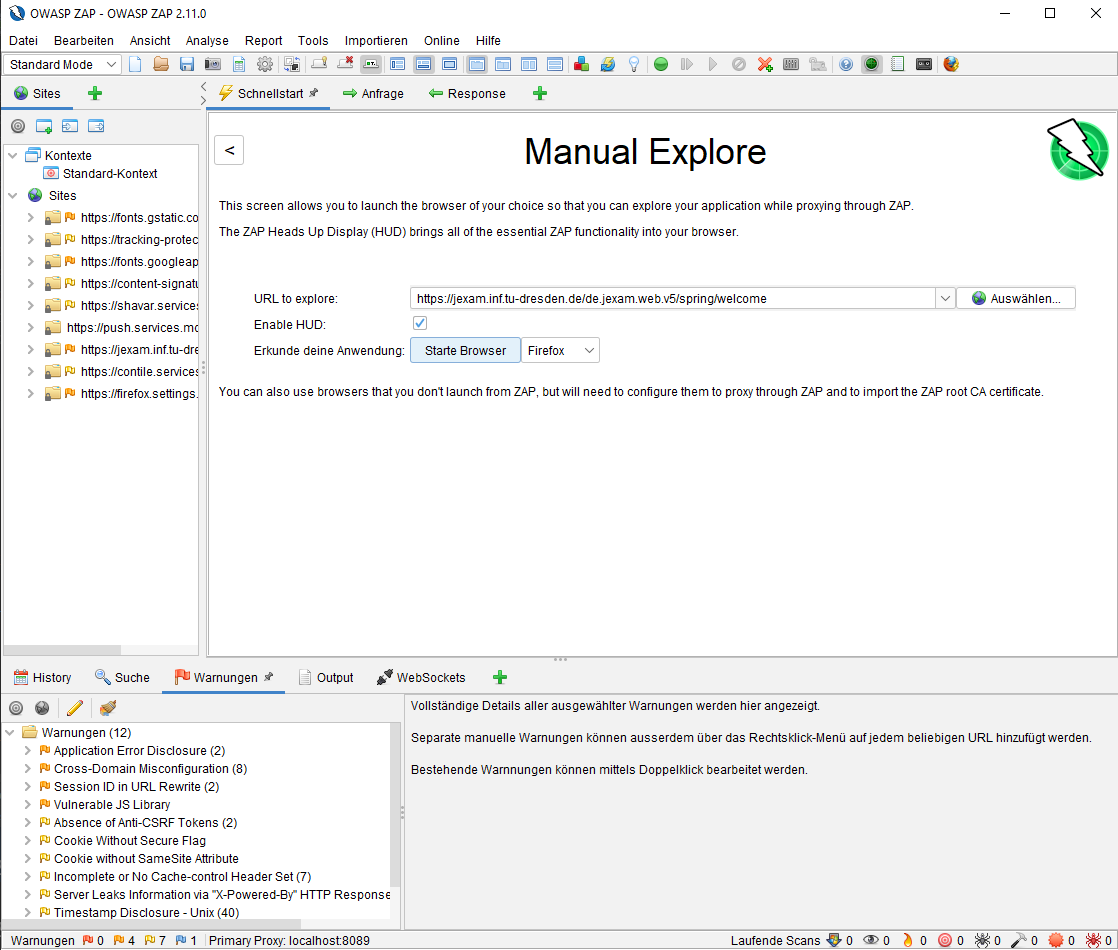
\includegraphics[scale=0.5]{images/zap-interface}
    \caption{Grafische Benutzeroberfläche von Zap} \label{fig:zap-interface}
\end{figure}



\subsection{Tests und Ergebnisse}

Die Testinfrastruktur von jExam wurde mit Docker unter Verwendung
von docker-compose entwickelt. Dies bietet die Möglichkeit, die
Testdienste in verschiedene Container aufzuteilen (dieses Konzept
wird in den nächsten Kapiteln ausführlich behandelt). Zu den
Testdiensten gehört auch ein Container, der speziell für Sicherheitstests
vorgesehen ist und automatisch bestimmte Befehle ausführt, um eine Version
von jExam zu scannen. Zunächst ist es notwendig, einige Begriffe zu
erklären, die im Folgenden verwendet werden.

\subsubsection{ZAP Spider}

Der Spider ist ein Werkzeug, das dazu dient, automatisch neue
Ressourcen (URLs) auf einer bestimmten Seite zu entdecken.
Er beginnt mit einer Liste von zu besuchenden URLs, den
sogenannten Seeds, die davon abhängen, wie der Spider gestartet
wird. Der Spider besucht dann diese URLs, identifiziert alle
Hyperlinks auf der Seite und fügt sie der Liste der zu besuchenden
URLs hinzu, und der Prozess wird rekursiv fortgesetzt, solange neue
Ressourcen gefunden werden (vgl. \cite{spider}). Dieser Prozess kann
Stunden dauern, je nachdem, wie viele Seiten und Links die Website
hat. Aus diesem Grund wird er oft mit einer Zeitbegrenzung durchgeführt.

\subsubsection{\acs{ajax} Spider}

Der \acs{ajax} Spider ist ein Add-on für einen Crawler namens Crawljax.
Das Add-on richtet einen lokalen Proxy in ZAP ein, um mit Crawljax
zu kommunizieren. Mit dem \acs{ajax} Spider ist es möglich Webanwendungen,
die  \acs{ajax} benutzen, in weit größerer Tiefe \Gls{crawlen} (Prozess der
automatischen Entdeckung neuer Ressourcen in einer Anwendung) als mit
dem nativen Spider. \acs{ajax} ist eine Reihe von Webentwicklungstechniken, die
verschiedene Webtechnologien auf der Client-Seite verwenden, um
asynchrone Webanwendungen zu erstellen. Mit \acs{ajax} können Webanwendungen
asynchron (im Hintergrund) Daten von einem Server senden und abrufen,
ohne die Anzeige und das Verhalten der bestehenden Seite zu beeinträchtigen.
Diese Computerarchitektur ermöglicht den Aufbau von Webanwendungen und
dynamischen, interaktiven Webseiten.\acs{ajax} spider wird beim Testen von Webanwendungen
empfohlen, die \acs{ajax} nutzen. Für eine vollständige Abdeckung einer
Webanwendung (z. B. um HTML-Kommentare abzudecken) soll auch den
nativen Spider verwendet werden (vgl. \cite{ajax}).

\subsubsection{Passive Scanning}

Passive Scanning ist eine Methode zur Erkennung von Schwachstellen, die auf
Informationen basiert, die aus Netzwerkdaten gesammelt werden. Beim Sammeln
dieser Informationen gibt es keine direkte Interaktion mit der Zielanwendung
(deshalb passiv). Beim passiven Scannen wird der gesamte Datenverkehr zwischen
dem Browser und der Website gelesen und aufgezeichnet, d. h. die POSTs/GETs
und ihre Antworten. ZAP analysiert diese Daten und sucht in seiner
Angriffsbibliothek nach bekannten Problemen. Passives Scannen führt keine
Angriffe aus und wird daher als harmlos angesehen. Beim passiven Scannen
können viele mögliche Fehler und Schwachstellen in einer Webanwendung
entdeckt werden.  Zu den bekanntesten gehören :

\begin{enumerate}
    \item Cross Domain Script Inclusion
    \item Cross Domain Misconfiguration
    \item X-Debug-Token Information Leak
    \item Username Hash Found
    \item Insecure Authentication
    \item Information Disclosure: Suspicious Comments
    \item Information Disclosure: Referrer
    \item Information Disclosure: In URL
    \item Information Disclosure: Debug Errors
    \item CSRF Countermeasures
\end{enumerate}

Diese Sicherheitslücken werden in dieser Arbeit nicht näher erläutert.
Informationen zu diesen Sicherheitslücken sind jedoch auf der Website von Zap Proxy
zu finden (vgl. \cite{passiv}).
\subsubsection{Active Scanning}

Active Scanning ist eine Methode zur Erkennung von Schwachstellen, bei
der versucht wird, potenzielle Schwachstellen mithilfe bekannter Angriffe
auf ausgewählte Ziele zu finden. Im Gegensatz zum passiven Scanning ist es
nicht risikolos. Es kann potenziell zu schwerwiegenden Problemen auf einem
Webserver führen. Aus diesem Grund wird Testern empfohlen, es nur für ihre
eigenen Anwendungen zu verwenden. Active Scanning ermöglicht es, mehrere
große Sicherheitslücken zu entdecken, die in einer Anwendung vorhanden
sein können. Zu den bekanntesten gehören :

\begin{enumerate}
    \item SQL Injection
    \item Directory Browsing
    \item CRLF Injection
    \item Cross Site Scripting (persistent und Reflected)
    \item Command Injection
    \item .htaccess Information Leak
\end{enumerate}

Es gibt auch viele andere, die in dieser Arbeit nicht behandelt werden.
Informationen zu diesen Sicherheitslücken sind jedoch auf der Website
von Zap Proxy zu finden (vgl. \cite{activ}).




Auf der jExam-Plattform wurden zwei Skripte für ihre Ausführung
implementiert. Es handelt sich dabei um die Skripte ZAP Baseline und
ZAP Full scan.  Da es zwei Versionen von jExam gibt, muss bei der
Ausführung der Skripte entschieden werden, welche der beiden Plattformen
getestet werden soll.

\subsubsection{ZAP Baseline}

Dieses Skript führt zuerst einen ZAP-Spider und dann ein Passiv Scanning
anhand der Daten aus dem Spider aus. Dies ist ein schneller und gründlicher
Prozess, der es ermöglicht, schnell zu erkennen, ob es ernsthafte
Schwachstellen gibt, die leicht ausgenutzt werden können. Schließlich erstellt
das Skript einen Bericht (siehe \Cref{fig:baseline}), der von den Testern sorgfältig geprüft werden muss.
Das Skript führt keinen echten ``Angriff'' durch und läuft nur für eine
relativ kurze Zeit (höchstens ein paar Minuten).


\begin{lstlisting}[language=Dockerfile,label={lst:baseline},caption={ZAP Baseline Ausführungsbefehl}]
command: [ "./wait-for-it.sh", "web:8080", "bash" ,"-c",
"zap-baseline.py -t http://web:8080 -r owaspReport.html" ]

# Web:8080: URL der Neuen Version von jExam, die sich im
Container namens Web befindet.
# ./wait-for-it.sh: Script, das einen Healt-Check
ausführt, um herauszufinden, ob die parametrisierte
Anwendung (In diesem Fall Web:8080) bereits gestartet ist.
# owaspReport.html: Webseite, die am Ende
der Testdurchführung generiert wird.
\end{lstlisting}

\subsubsection{ZAP Fullscan}


Dieses Skript führt einen ZAP Spider für eine unbestimmte Zeit aus.
Je mehr Ressourcen und Hyperlinks die Anwendung besitzt, desto länger
dauert dieser Prozess. Danach wird ein Ajax Spider ausgeführt, der
ebenfalls für eine unbestimmte Zeit ausgeführt wird. Danach wird ein
Full Active Scan ausgeführt und schließlich ein Bericht erstellt
(siehe \Cref{fig:baseline}),auf  den der Tester zugreifen kann.
Das Skript führt echte "Angriffe" aus  und kann potenziell über einen
längeren Zeitraum (mehrere Stunden) laufen. Das Skript ist jedoch viel
effizienter und findet mehr  Sicherheitslücken als ZAP Baseline.

\begin{lstlisting}[language=Dockerfile,label={lst:fullscan},caption={ZAP Fullscan Ausführungsbefehl}]
command: [ "./wait-for-it.sh", "web:8080", "bash" ,"-c",
"zap-full-scan.py -d -j -m 1 -t http://web:8080 -r owaspReport.html" ]

\end{lstlisting}


\begin{figure}[H]
    \centering
    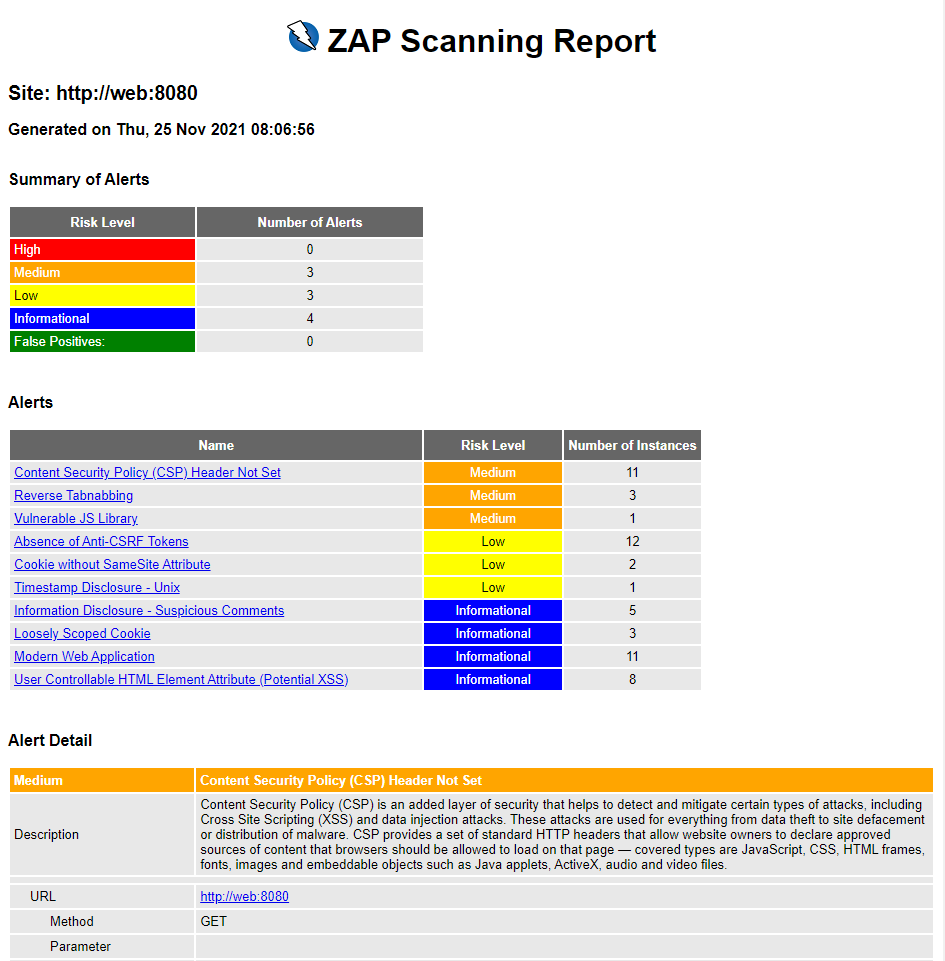
\includegraphics[scale=0.5]{images/zap-report}
    \caption{Bericht nach der Ausführung einer Zap Baseline} \label{fig:baseline}
\end{figure}




Die Sicherheit einer Anwendung zu testen ist eine schwierige Aufgabe,
aber Werkzeuge wie Zap machen die Tür zu diesem Bereich der Programmierung
immer kleiner. Mit Hilfe der Scanner ist es möglich, Sicherheitslücken zu
finden, die den Entwicklern ermöglichen, sie zu beheben. Dadurch wird eine
gute Softwarequalität für die Zukunft gewährleistet.









